\documentclass[a4paper, 14pt]{extarticle}

% Поля
%----------------------
\usepackage{geometry}
\geometry{a4paper,left=2cm,right=1cm,
    top=2cm,bottom=2cm,bindingoffset=0cm}
%----------------------

% Russian-specific packages
%----------------------
\usepackage[T2A]{fontenc}
\usepackage[utf8]{inputenc}
\usepackage[english, main=russian]{babel}
%----------------------

\usepackage{textcomp}

% Красная строка
%----------------------
\usepackage{indentfirst}
%----------------------

% Graphics
%----------------------
\usepackage{graphicx}
\graphicspath{ {./images} }
\usepackage{wrapfig}
%----------------------

% Import minted
%----------------------
\usepackage{minted}
%----------------------

% Tables

%----------------------
\usepackage{longtable}
\usepackage{ragged2e}
\usepackage{booktabs}
\usepackage{array}
\usepackage{caption}
\usepackage{float}

%----------------------

\linespread{1.3}
\sloppy
\clubpenalty=10000
\widowpenalty=10000

\begin{document}

%--------------------------------------
%			ТИТУЛЬНЫЙ ЛИСТ
%--------------------------------------
\begin{titlepage}
\thispagestyle{empty}
\newpage


%Шапка титульного листа
%--------------------------------------
\vspace*{-60pt}
\hspace{-65pt}
\begin{minipage}{0.3\textwidth}
\hspace*{-20pt}\centering

\includegraphics[width=\textwidth]{emblem}
\end{minipage}
\begin{minipage}{0.67\textwidth}\small \textbf{
\vspace*{-0.7ex}
\hspace*{-6pt}\centerline{Министерство науки и высшего образования Российской Федерации}
\vspace*{-0.7ex}
\centerline{Федеральное государственное бюджетное образовательное учреждение }
\vspace*{-0.7ex}
\centerline{высшего образования}
\vspace*{-0.7ex}
\centerline{<<Московский государственный технический университет}
\vspace*{-0.7ex}
\centerline{имени Н.Э. Баумана}
\vspace*{-0.7ex}
\centerline{(национальный исследовательский университет)>>}
\vspace*{-0.7ex}
\centerline{(МГТУ им. Н.Э. Баумана)}}
\end{minipage}
%--------------------------------------

%Полосы
%--------------------------------------
\vspace{-25pt}
\hspace{-35pt}\rule{\textwidth}{2.3pt}

\vspace*{-20.3pt}
\hspace{-35pt}\rule{\textwidth}{0.4pt}
%--------------------------------------

\vspace{1.5ex}
\hspace{-35pt} \noindent \small ФАКУЛЬТЕТ\hspace{80pt} <<Информатика и системы управления>>

\vspace*{-16pt}
\hspace{47pt}\rule{0.83\textwidth}{0.4pt}

\vspace{0.5ex}
\hspace{-35pt} \noindent \small КАФЕДРА\hspace{50pt} <<Теоретическая информатика и компьютерные технологии>>

\vspace*{-16pt}
\hspace{30pt}\rule{0.866\textwidth}{0.4pt}
  
\vspace{11em}

\begin{center}
\Large {\bf Лабораторная работа №3} \\ 
\large {\bf по курсу <<Базы данных>>} \\

% Labname
\large <<Преобразование модели «сущность-связь» в реляционную модель>> \\
\end{center}\normalsize

\vspace{8em}


\begin{flushright}
  {Студент группы ИУ9-51Б Киселев К.А. \hspace*{15pt}\\ 
  \vspace{2ex}
  Преподаватель Вишняков И.Э. \hspace*{15pt}}
\end{flushright}

\bigskip

\vfill
 

\begin{center}
\textsl{Москва 2023}
\end{center}
\end{titlepage}
%--------------------------------------
%		КОНЕЦ ТИТУЛЬНОГО ЛИСТА
%--------------------------------------

\newpage




\section{Постановка задачи}

\begin{enumerate}
	\item{Преобразовать модель «сущность-связь», созданную в лабораторной работе №1, в реляционную модель согласно процедуре преобразования.} 
	\item{Обосновать выбор типов данных, ключей, правил обеспечения ограничений минимальной кардинальности.}
\end{enumerate}

\newpage

\section{Практическая реализация}

В соответствии с правилами преобразования, из созданной ранее модели сущность-связь, получили реляционную модель, представленную на  рисунке \ref{fig:relation_model}.

\begin{figure}[ht]
\centering
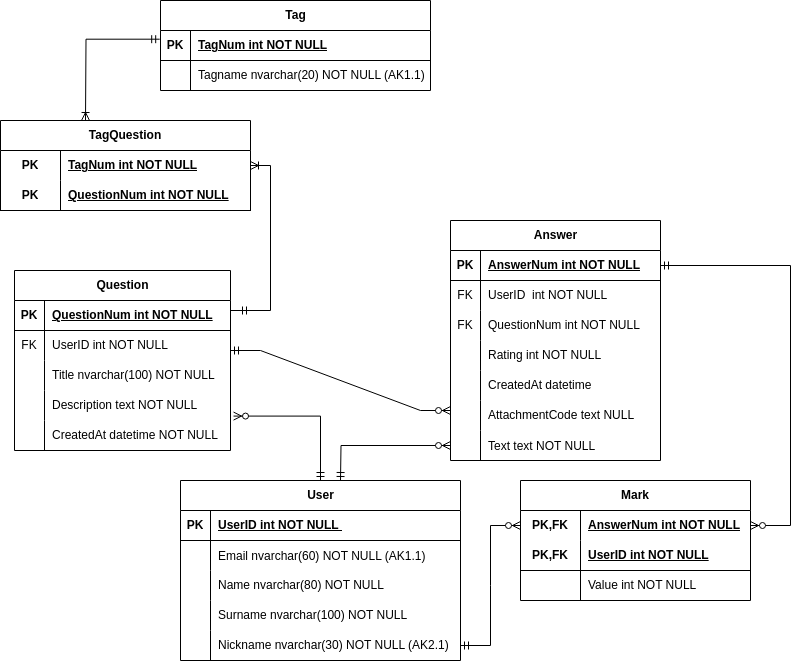
\includegraphics[width=0.6\textwidth]{Diagram2}
\caption{Реляционная модель.} 
\label{fig:relation_model}
\end{figure}

На рисунке \ref{fig:er_model} представлена созданная в лабораторной работе №1 модель “Сущность-связь”

\begin{figure}[ht]
\centering
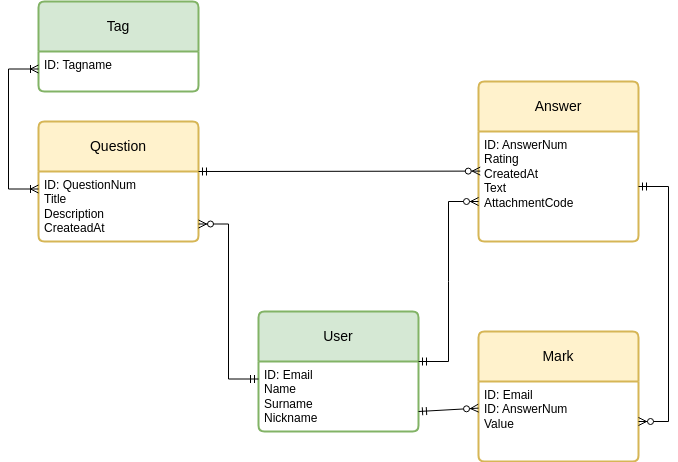
\includegraphics[width=0.6\textwidth]{Diagram1} 
\caption{Модель “Сущность-связь”} 
\label{fig:er_model}
\end{figure}


\subsection{Описание сущностией}

Были реализованы таблицы для каждой сущности. В таблцие \ref{tab:user_tab} представлены типы данных и их значения по умолчанию для сущности User

\begin{table}[H]
\centering
\caption{Сущность User}
\label{tab:user_tab}
\setlength\extrarowheight{2pt}
\begin{tabular}{|c|c|c|c|c|}
\hline
\textbf{Column Name} & \textbf{Type} & \textbf{Key} & \textbf{NULL Status} & \textbf{Remarks} \\
\hline
UserID & int & Primary & NOT NULL & Surrogate Key \\
\hline
Email & nvarchar (256) & Alternate & NOT NULL & Unique (AK1.1) \\
\hline
Name & nvarchar (80) & No & NOT NULL & \\
\hline
Surname & nvarchar (100) & No & NOT NULL & \\
\hline
Nickname & nvarchar(30) & Alternate & NOT NULL & Unique (AK2.1) \\
\hline
\end{tabular}
\end{table}


В таблцие \ref{tab:question_tab} представлены типы данных и их значения по умолчанию для сущности Question

\begin{table}[H]
\centering
\caption{Таблица Question}
\label{tab:question_tab}
\setlength\extrarowheight{2pt}
\begin{tabular}{|c|c|c|c|c|}
\hline
\textbf{Column Name} & \textbf{Type} & \textbf{Key} & \textbf{NULL Status} & \textbf{Remarks} \\
\hline
QuestionNum & int & Primary & NOT NULL & Surrogate Key \\
\hline
UserID & int & Foreign & NOT NULL & \\
\hline
Title & nvarchar (100) & No & NOT NULL & \\
\hline
Description & nvarchar(max) & No & NOT NULL & \\
\hline
CreatedAt & datetime & No & NOT NULL & \\
\hline
\end{tabular}
\end{table}

\newpage

В таблцие \ref{tab:answer_tab} представлены типы данных и их значения по умолчанию для сущности Answer

\begin{table}[H]
\centering
\caption{Таблица Answer}
\label{tab:answer_tab}
\setlength\extrarowheight{2pt}
\begin{tabular}{|c|c|c|c|c|}
\hline
\textbf{Column Name} & \textbf{Type} & \textbf{Key} & \textbf{NULL Status} & \textbf{Remarks} \\
\hline
AnswerNum & int & Primary & NOT NULL & Surrogate Key \\
\hline
UserID & int & Foreign & NOT NULL & \\
\hline
QuestionNum & int & Foreign & NOT NULL & \\
\hline
Rating & int & No & NOT NULL & \\
\hline
AttachmentCode & nvarchar(max) & No & NULL & \\
\hline
Text & nvarchar(max) & No & NOT NULL & \\
\hline
CreatedAt & datetime & No & NOT NULL & \\
\hline
\end{tabular}
\end{table}


В таблцие \ref{tab:tag_tab} представлены типы данных и их значения по умолчанию для сущности Tag

\begin{table}[H]
\centering
\caption{Таблица Tag}
\label{tab:tag_tab}
\setlength\extrarowheight{2pt}
\begin{tabular}{|c|c|c|c|c|}
\hline
\textbf{Column Name} & \textbf{Type} & \textbf{Key} & \textbf{NULL Status} & \textbf{Remarks} \\
\hline
TagNum & int & Primary & NOT NULL & Surrogate Key \\
\hline
Tagname & nvarchar(20) & Alternate & NOT NULL & Unique (AK1.1) \\
\hline
\end{tabular}
\end{table}


В таблцие \ref{tab:mark_tab} представлены типы данных и их значения по умолчанию для сущности Question

\begin{table}[H]
\centering
\caption{Таблица Mark}
\label{tab:mark_tab}
\setlength\extrarowheight{2pt}
\begin{tabular}{|c|c|c|c|c|}
\hline
\textbf{Column Name} & \textbf{Type} & \textbf{Key} & \textbf{NULL Status} & \textbf{Remarks} \\
\hline
AnswerNum & int & Primary, Foreign & NOT NULL & \\
\hline
UserID & int & Primary, Foreign & NOT NULL & \\
\hline
Value & int & No & NOT NULL & \\
\hline
\end{tabular}
\end{table}

\newpage

В таблцие \ref{tab:tag_question_tab} представлены типы данных и их значения по умолчанию для таблицы TagQuestion

\begin{table}[H]
\centering
\caption{Таблица TagQuestion}
\label{tab:tag_question_tab}
\setlength\extrarowheight{2pt}
\begin{tabular}{|c|c|c|c|c|}
\hline
\textbf{Column Name} & \textbf{Type} & \textbf{Key} & \textbf{NULL Status} & \textbf{Remarks} \\
\hline
QuestionNum & int & Primary, Foreign & NOT NULL & \\
\hline
TagNum & int & Primary, Foreign & NOT NULL & \\
\hline
\end{tabular}
\end{table}



\pagebreak

\subsection{Обоснование правил обеспечения ограничений минимальной кардинальности}

Обоснование правил обеспечения ограничений минимальной кардинальности приведено на следующих таблицах:


User к Question не идентифицирующая связь — M-O 1:N;


\begin{table}[H]
\centering
\caption{User к Question}
\begin{tabular}{|>{\centering\arraybackslash}m{4cm}|>{\RaggedRight}m{6cm}|>{\RaggedRight}m{6cm}|}
\hline
\textbf{USER Обязательный родитель} & \textbf{Действия для USER (родитель)} & \textbf{Действия для QUESTION (ребенок)} \\
\hline
Вставка & — & Получение родителя. \\
\hline
Изменение первичного или внешнего ключа & Запрещено — суррогатный ключ. & Запрещено — автор вопроса не может меняться. \\
\hline
Удаление & Каскадное удаление ребенка. & — \\
\hline
\end{tabular}
\end{table}

User к Answer не идентифицирующая связь — M-O 1:N;

\begin{table}[H]
\centering
\caption{User к Answer}
\setlength\extrarowheight{2pt} % Дополнительное пространство между строками
\begin{tabular}{|>{\centering\arraybackslash}m{4cm}|>{\RaggedRight\arraybackslash}m{6cm}|>{\RaggedRight\arraybackslash}m{6cm}|}
\hline
\textbf{USER Обязательный родитель} & \textbf{Действия для USER (родитель)} & \textbf{Действия для ANSWER (ребенок)} \\
\hline
Вставка & — & Получение родителя. \\
\hline
Изменение первичного или внешнего ключа & Запрещено — суррогатный ключ. & Запрещено — автор ответа не может меняться. \\
\hline
Удаление & Каскадное удаление ребенка. & — \\
\hline
\end{tabular}
\end{table}

\newpage

User к Mark идентифицирующая связь — M-O 1:N;

\begin{table}[H]
\centering
\caption{User к Mark}
\setlength\extrarowheight{2pt} % Дополнительное пространство между строками
\begin{tabular}{|>{\centering\arraybackslash}m{4cm}|>{\RaggedRight\arraybackslash}m{6cm}|>{\RaggedRight\arraybackslash}m{6cm}|}
\hline
\textbf{USER Обязательный родитель} & \textbf{Действия для USER (родитель)} & \textbf{Действия для MARK (ребенок)} \\
\hline
Вставка & — & Получение родителя. \\
\hline
Изменение первичного или внешнего ключа & Запрещено — суррогатный ключ. & Запрещено — автор оценки не может меняться. \\
\hline
Удаление & Каскадное удаление ребенка. & — \\
\hline
\end{tabular}
\end{table}

\newpage

Tag к TagQuestion идентифицирующая связь — M-M 1:N;

\begin{table}[H]
\centering
\caption{Tag к TagQuestion}
\begin{tabular}{|>{\centering\arraybackslash}m{4cm}|>{\RaggedRight}m{6cm}|>{\RaggedRight}m{6cm}|}
\hline
\textbf{TAG Обязательный родитель} & \textbf{Действия для TAG (родитель)} & \textbf{Действия для TAGQUESTION (ребенок)} \\
\hline
	Вставка & Вставка с помощью транзакции. После вставки Tag необходимо вставить в TagQuestion строку $(TagNum, QuestionNum)$, где TagNum - идентификатор вставленного тега, QuestionNum- идентификатор связанного вопроса& Получение родителя. \\
\hline
Изменение первичного или внешнего ключа & Запрещено — суррогатный ключ. & Запрещено — сопряжение. \\
\hline
Удаление & Каскадное удаление ребенка. & Возможно, если при этом удаляемая строка была единственной ссылающейся на TagNum, то удаляется и Tag с соответствующим TagNum \\
\hline
\end{tabular}
\end{table}

\pagebreak

Question к TagQuestion идентифицирующая связь — M-M 1:N;

\begin{table}[H]
\centering
\caption{Question к TagQuestion}
\begin{tabular}{|>{\centering\arraybackslash}m{4cm}|>{\RaggedRight}m{6cm}|>{\RaggedRight}m{6cm}|}
\hline
\textbf{QUESTION Обязательный родитель} & \textbf{Действия для QUESTION (родитель)} & \textbf{Действия для TAGQUESTION (ребенок)} \\
\hline
	Вставка & Вставка с помощью транзакции. После вставки нового вопроса, небходимо добавить в TagQuestion строки вида $(TagNum_i, QuestionNum)$, где $QuestionNum$ идентификатор вставленного вопроса & Получение родителя. \\
\hline
Изменение первичного или внешнего ключа & Запрещено — суррогатный ключ. & Запрещено — сопряжение. \\
\hline
Удаление & Каскадное удаление ребенка. & Возможно только при условии, что остались другие строки таблицы соответствующие тому же вопросу\\
\hline
\end{tabular}
\end{table}

\newpage

Answer к Mark идентифицирующая связь — M-O 1:N;

\begin{table}[H]
\centering
\caption{Answer к Mark}
\begin{tabular}{|>{\centering\arraybackslash}m{4cm}|>{\RaggedRight}m{6cm}|>{\RaggedRight}m{6cm}|}
\hline
\textbf{ANSWER Обязательный родитель} & \textbf{Действия для ANSWER (родитель)} & \textbf{Действия для MARK (ребенок)} \\
\hline
Вставка & — & Получение родителя. \\
\hline
Изменение первичного или внешнего ключа & Запрещено — суррогатный ключ. & Запрещено — ответ, на который была поставлена оценка, не может меняться. \\
\hline
Удаление & Каскадное удаление ребенка. & — \\
\hline
\end{tabular}
\end{table}


Question к Answer не идентифицирующая связь — M-O 1:N;

\begin{table}[H]
\centering
\caption{Question к Answer}
\begin{tabular}{|>{\centering\arraybackslash}m{4cm}|>{\RaggedRight}m{6cm}|>{\RaggedRight}m{6cm}|}
\hline
\textbf{QUESTION Обязательный родитель} & \textbf{Действия для QUESTION (родитель)} & \textbf{Действия для ANSWER (ребенок)} \\
\hline
Вставка & — & Получение родителя. \\
\hline
Изменение первичного или внешнего ключа & Запрещено — суррогатный ключ. & Запрещено — вопрос, на который дан ответ не может, меняться. \\
\hline
Удаление & Каскадное удаление ребенка. & — \\
\hline
\end{tabular}
\end{table}



\end{document}
